\chapter{Introduction}
\label{chap:introduction}
\emph{In the introductory chapter, some basic aspects of virtualization will pass the revue.}
\section{Virtualization}

\subsection{Abstractions}

Computer systems are built as hierarchies with interfaces that separate levels of abstraction. Those levels of abstraction hide lower-level implementation details, which allows for independant development of each seperate layer and thus simplifying the development and maintanance process \citep{ArchVM}.

To clearify this layered build of computer systems, two examples are provided: one applies to application design, whereas the second example applies to disk storage.
\paragraph{First example} Imaging a higher-level programming language, called \textbf{Language1}. This language consists of classes, methods, variables, etc\ldots . This Language5 is very convenient and understandable for people. However, since computer systems only understand machine language, let us call this \textbf{Language1}, one cannot simply feed this language to the low-level digital circuits and hoping for the program to execute.

In fact, the gap between what is conventient for people and what is convenient for computers tend to be very large. So the need to translate the higher-level code (Language5) to low-level bytecode (Language1) is needed. This is where abstractation layers come in.

Imaging a virtual machine \textbf{Machine1} that accepts Language5. The programs written in Language5 can then be translated of interpreted by a program written in Language1, which can be directly executed on the computer hardware \citep{Tanenbaum}.

However, for practical reasons, those two languages Language5 and Language1 cannot be too different. This means that intermediate Languages and thus virtual machines must exist to interpret of translate Language5 into a more lower-level language \textbf{Language4}. This process of continually and gradually translating higher-level languages into lower-level languages can further be executed until the final, lowest-level language (Language0) is reached  \citep{Tanenbaum}. \\ \\
Each virtual machine is a layer. So in the example given, 5 layers exist to translate a higher-level language into a lower-level one. The bottom-most language is the simplest one that computers understand (i.e.: bytecode) whereas the top-most language is the most sophisticated one.

\paragraph{Second example}

In the case of hard disk abstraction, the operating systems hides (i.e.: abstracts) the addressing details, that is, sectors and tracks, for the application software. This means that, from the application point-of-view, the disk appears as a set of files.

Programmers create, read, modify and delete files without knowing those low-level tracks and sectors. The figure below clearyfies the process.

\begin{figure}[h]
    \centering
    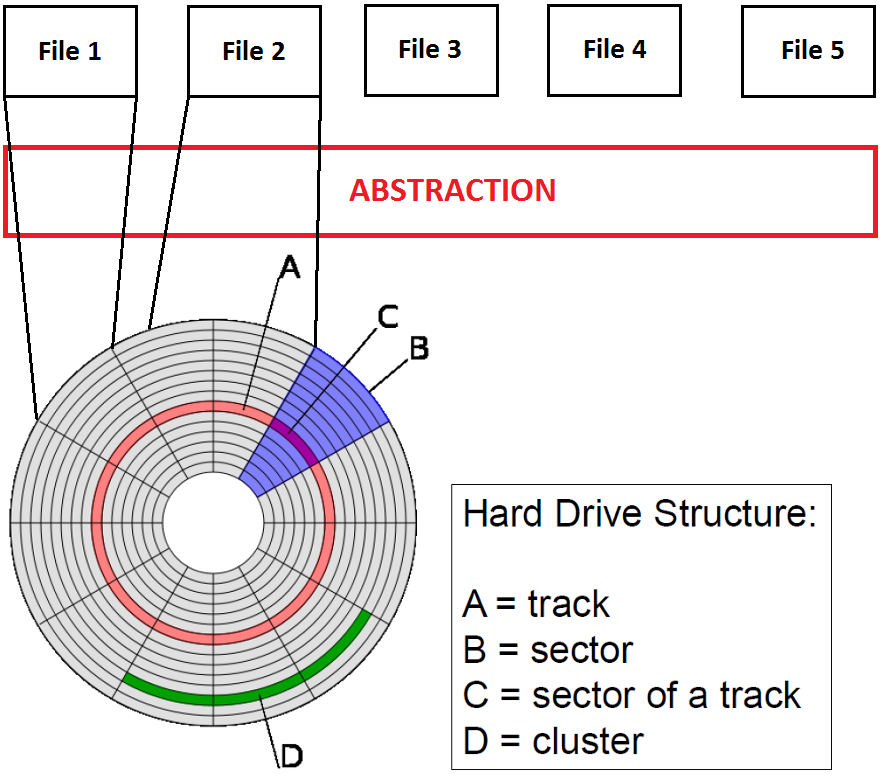
\includegraphics[width=0.65\textwidth]{HD_struct.png}
    \caption[Abstraction applied to disk storage]{Abstraction applied to disk storage. The abstraction layer is in fact the operating system.}
\end{figure}

\clearpage

In fact, not only computer systems are built as hierarchies: also networking systems use several abstractation layers to communicate with each other. What follows is a brief explanation of the OSI model, that describes how network applications may communicate with each other \citep{OSI}.

The OSI model consists of 7 layers as illustrated in the figure below:
\begin{figure}[h]
    \centering
    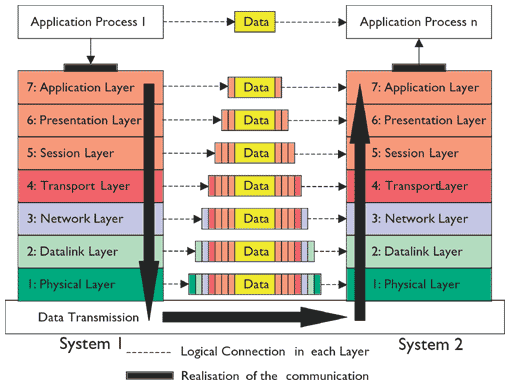
\includegraphics[width=0.65\textwidth]{OSI.png}
    \caption[The OSI model]{The OSI model is another example of abstraction. This time not in computer systems, but in networking.}
\end{figure}
Top-level applications do not communicate directly with each other. Instead, data is passed from one layer to another, starting at the application layer and proceeding to the bottom layer. There, the data is sent over the communication channel to the other host where the whole process takes place in reverse order \citep{OSI2}. 

The seven layers can be seen as abstraction layers. Each layer hides details of the level directly beneith it.

\subsection{Abstraction and virtual machines}

Virtualization exists in many forms. Not only there exist storage (disk) virtualization, but also network virtualization, virtualized applications and hypervisors. In the first case, virtualization does not necessarily aim to hide details \citep{ArchVM}. 

Consider the figure below. Virtualization transforms a physical disk into two smaller disks. Each of those disks appears to have its own tracks, sectors and clusters. Furthermore, the virtualization software uses the file abstraction described in the previous section to map a virtual disk onto the real physical disk.

Data that is to be written onto the virtual disk, is converted to a file write. Since the file resides on the real physical disk, data is actually written to the physical disk.

This is an example of abstraction and virtualization applied to disk storage.
\begin{figure}[h]
    \centering
    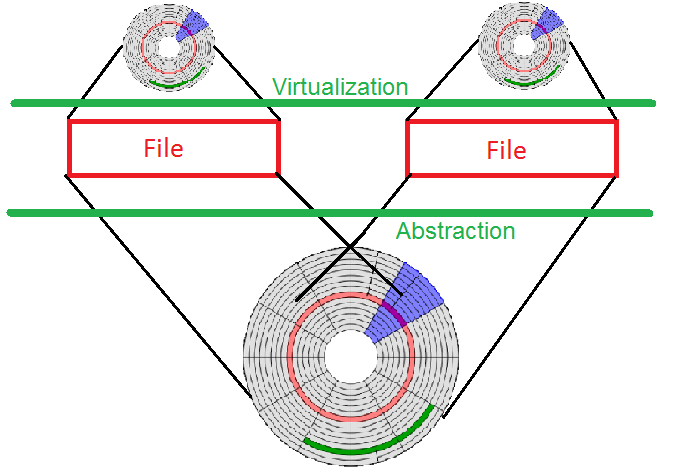
\includegraphics[width=0.65\textwidth]{HD.png}
    \caption[Virtualization of hard disks]{Virtualization applied to disk storage}
\end{figure}
Obviously, the whole concept of (disk) virtualization can also be applied to physical machines. This is where hypervisors make their entry.

A hypervisor will abstract the physical resources, that is, CPU, memory, disk and network, from systems running on top of it \citep{VMIntro1}. This means that those physical resources are shared between the virtual machines and thus allows that multiple virtual machines can run on a single physical machine.

Chapter \ref{chap:virtualnetworks} provides more details about virtualization and hypervisors in particular.

\section{Why use virtualization}

\subsection{Benefits of using machine virtualization}

\begin{itemize}
\item \textbf{Server consolidation} The most prominent advantage of using machine virtualization (where a hypervisor is used to abstract the physical machine resources) is server consolidation. In the case of a typical non-virtualized application server for example, about 5\% to 10\% of the server's hardware is utilized. However, when a server hosts multiple virtual machines, utilization can reach values of 50\% to 80\% \citep{Benefit1}.

The whole point of machine virtualization is that the hardware of the physical machine is used more efficiently. It permits to get more out of the existing, physical hardware, because multiple virtual machines that act as real servers can run on top of one physical machine. This has an important consequence: fewer physical servers can be used to achieve the same goals. This means lower operating costs, e.g.: less power and air conditioning are needed \citep{Benefit2}.
\item \textbf{Easy cloning} In contrast to a physical server, which consists of a mixture of application files, OS files, driver files and user files, a VM exists as a single file \citep{Benefit1}. This file can be duplicated, which leads to easy creation of exactly the same machine (server). Obviously, these images can be modified for each application \citep{Benefit3}.
\item \textbf{High availability} When running multiple virtual machines, the load can be distributed amongst them. When a VM fails, another VM can just be started with ensures minimal downtime or data loss \citep{Benefit3}.
\item \textbf{Scalability} Scalability can greatly be improved using virtual machines. Additional resources can quickly be allocated from the host to the guest \citep{Microsoft}: when a certain task requires more RAM, adding RAM to the virtual machine consist of editing a parameter on the hypervisor, whereas in the case of a physical machine, it can take minutes to add more RAM \citep{Benefit3}.
\end{itemize}

\subsection{Challenges and disadvantages of using machine virtualization}

\begin{itemize}
\item \textbf{Longer recovery in case of physical hardware failure} and therefore longer downtime. When the physical machine breaks down because of a catastrophic hardware failure, all the virtual machines need to wait until the physical host is brung up online, after which the VM's can start booting. This means increased downtime \citep{Benefit3}.
\end{itemize}


\section{Security issues regarding virtualization}
\label{sec:securityRegardingVirtualization}
Consider the VMware ESXi Hypervisor. All virtual machines are isolated from each other \citep{Benefit4}. The advantages of this practise are for example the fact that if one VM fails, the remaining VM's remain accessible or the fact that if one VM gets infected with, let's say, a Trojan Horse, this will not affect the other VM's \citep{CompTia}.

However, this is not entirely true: cases have been reported in where virusses are able to break out VM's \citep{Crossover}. Additionaly, since VM are networked - either internally using a virtual switch or bridged with the physical network (or both), a new thread arises. Malware with a network component (e.g.: worms), travels where their routing tells - or allows - them to go \citep{Stackex}. Therefore , it is perfectly possible that an infected VM might infect other VM's while the network administrator believed this could never happen.

The whole point is that one may not assume that VM's are really isolated from each other and that an infected VM cannot infect another one - even if they are not networked. Chapter 3 will cover security in more detail.\\

In this thesis, virtual networks will be tested against known and unknown security problems concerning virtual networks. Furthermore, securtity aspects will be highlighted in virtual networks. \\ \\
\emph{This chapter briefly described some basic concepts of virtualization, especially machine virtualization. Advantages and disadvantages of virtualization have been discussed as well as a brief mention about security issues related to virtualization.\\
In the next chapter, )}